\documentclass[xcolor=svgnames]{beamer}
\mode<presentation>
{
      \setbeamertemplate{footline}[page number]
      \setbeamercovered{transparent}
      \setbeamertemplate{navigation symbols}{}
      \usecolortheme[named=DarkGreen]{structure}
}

\usepackage[english]{babel}
\usepackage{times}
\usepackage{CJKutf8}
\usepackage{graphics}
\usepackage{color}
\usepackage{xcolor}
\usepackage{listings}

\usepackage{caption}
\DeclareCaptionFont{white}{\color{white}}
\DeclareCaptionFormat{listing}{\colorbox{gray}{\parbox{\textwidth}{#1#2#3}}}
\captionsetup[lstlisting]{format=listing,labelfont=white,textfont=white}

\begin{document}
\begin{CJK*}{UTF8}{gbsn}


\title{进程}

\author{李中国}
\institute{苏州大学计算机科学与技术学院}
%\date{2011年5月30日}
\date{}

\begin{frame}
  \titlepage
\end{frame}


\begin{frame}{进程概念}
\begin{itemize}
\item 操作系统执行用户程序
\begin{itemize}
\item 批处理系统 --- 作业
\item 分时系统 --- 用户程序、任务
\end{itemize}
\item 进程: 运行中的程序 
\item 进程包含三部分内容:
\begin{itemize}
\item 程序代码(text section)
\item 当前状态: 程序计数器(program counter)以及寄存器(registers)
\item 栈(函数参数, 返回地址, 局部变量)
\item 数据区(data section, 全局变量)
\item 堆(运行时动态分配的内存)
\end{itemize}
%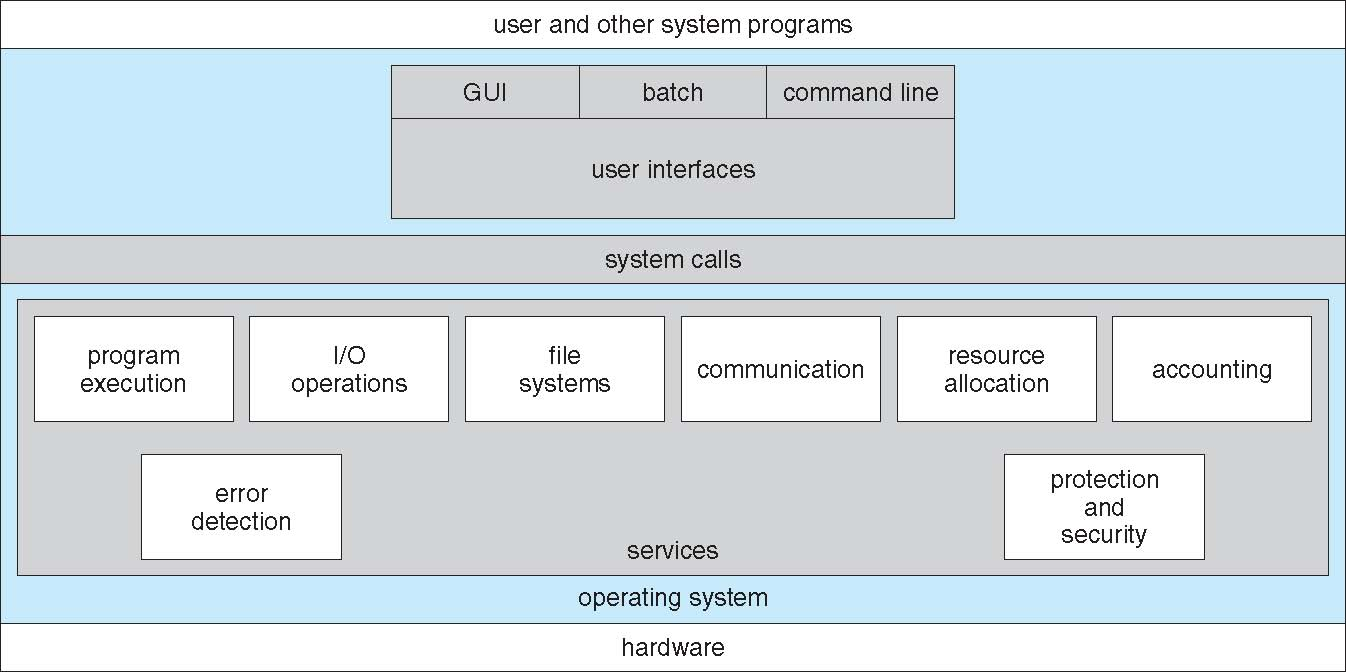
\includegraphics[width=1.0\textwidth]{services.jpg}
\end{itemize}
\end{frame}

\begin{frame}{内存中的进程结构}
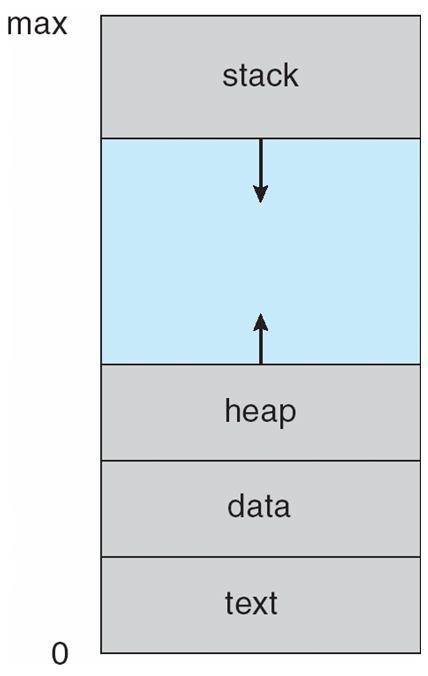
\includegraphics[width=0.5\textwidth]{process.png}
\end{frame}

\begin{frame}{进程的状态}
\begin{itemize}
\item new: 进程正在被创建当中
\item running: 进程的指令正在CPU上执行
\item waiting: 等待某事件的发生(e.g, I/O)
\item ready: 等待CPU
\item terminated: 进程终止
\end{itemize}
\end{frame}

\begin{frame}{进程状态迁移}
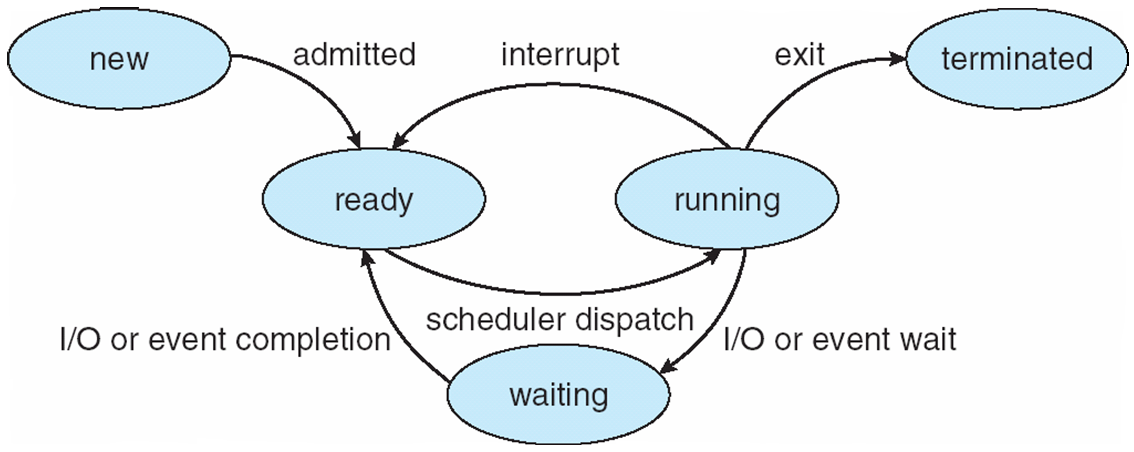
\includegraphics[width=1.0\textwidth]{state.png}
\end{frame}

\begin{frame}{进程控制块(PCB)}
\begin{columns}%[t]
\column{.5\textwidth}
用于存放与每个进程相关的信息
\begin{itemize}
\item 进程状态
\item 程序计数器PC
\item CPU寄存器
\item CPU调度信息
\item 内存管理信息
\item I/O状态信息
\item 记账信息
\end{itemize}
\column{.5\textwidth}
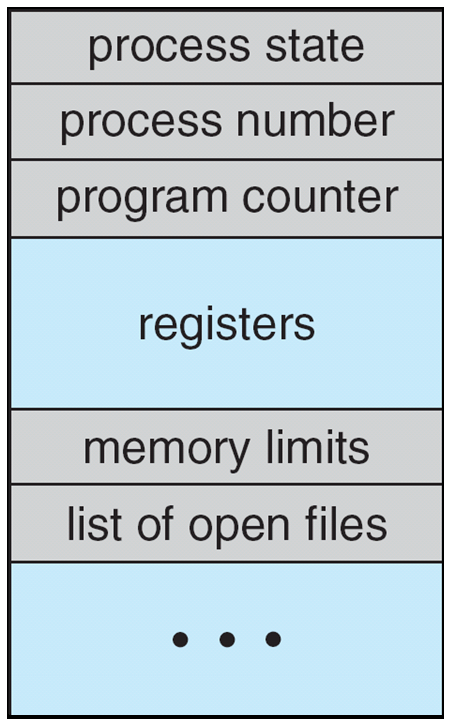
\includegraphics[width=0.6\textwidth]{PCB.png}
\end{columns}%[t]
\end{frame}

\begin{frame}{CPU在进程间切换}
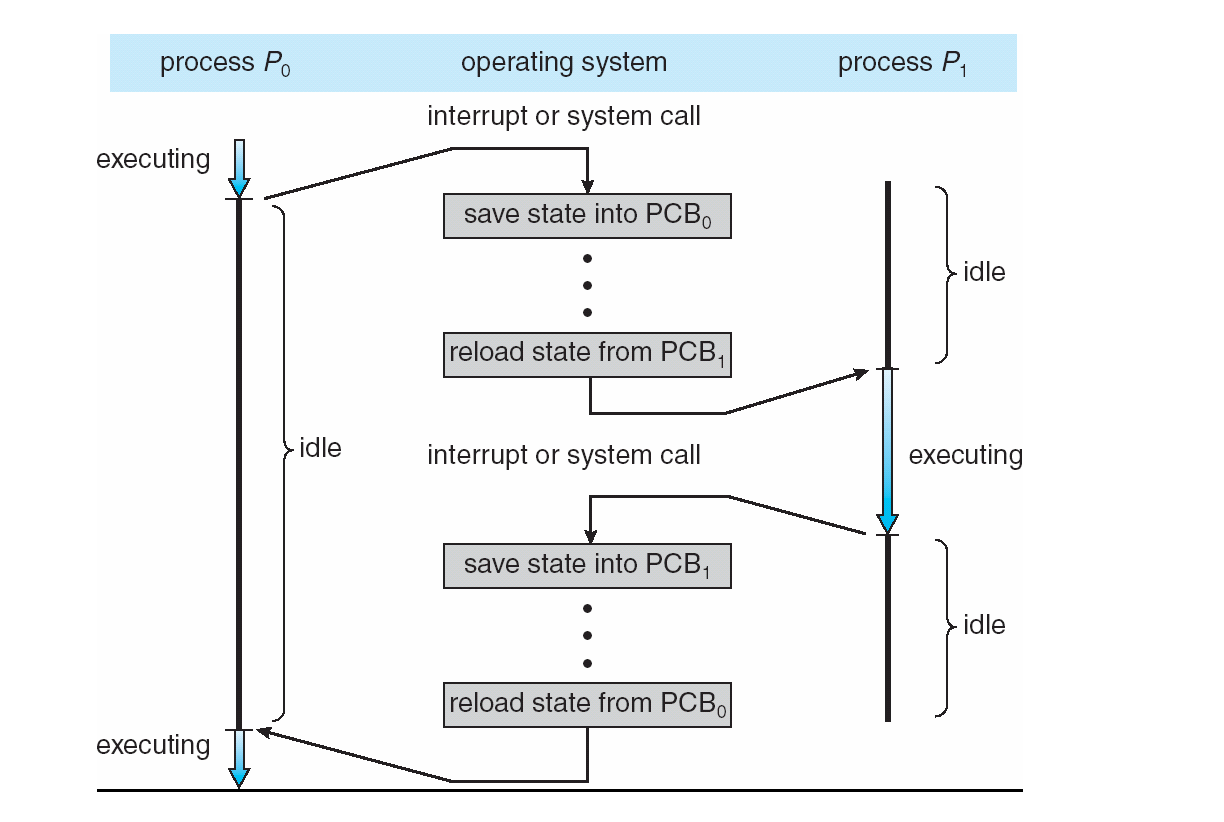
\includegraphics[width=1.0\textwidth]{switch.png}
\end{frame}

\begin{frame}{进程调度}
\begin{itemize}
\item 最大化CPU利用率; 实现分时系统
\item 进程调度器:从ready状态的进程中选择一个运行
\item 调度队列:
\begin{itemize}
\item 作业队列(Job queue) -- 系统中所有进程的集合
\item 就绪队列(ready queue) -- 内存中所有处于ready状态的进程
\item 设备队列(device queues) -- 等待某I/O设备的进程集合
\item 进程在上述队列之间来回迁移
\end{itemize}
\end{itemize}
\end{frame}

\begin{frame}{就绪队列及设备队列示意}
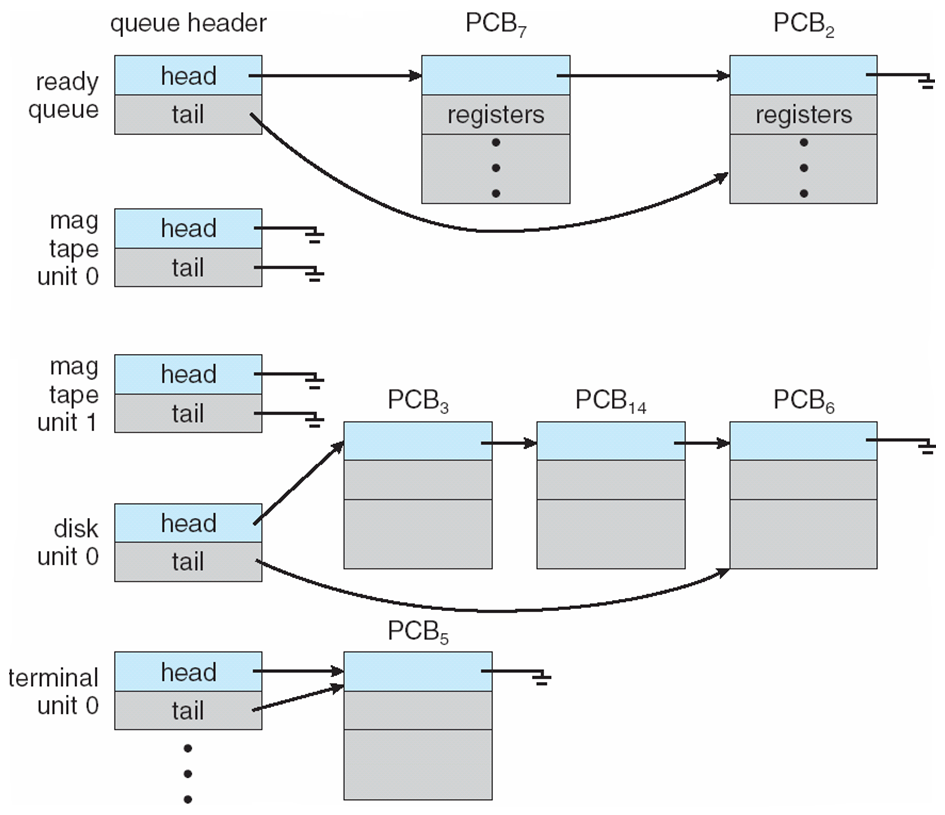
\includegraphics[width=0.8\textwidth]{queues.png}
\end{frame}

\begin{frame}{进程调度示意图}
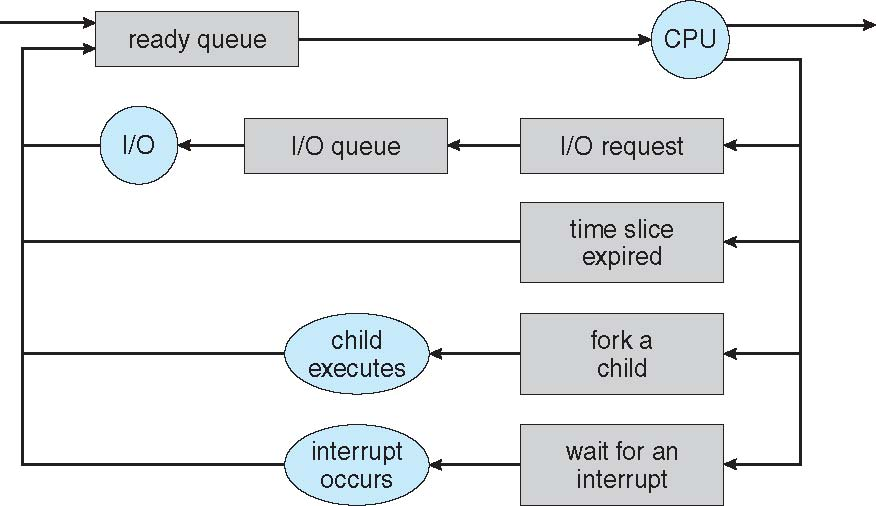
\includegraphics[width=0.8\textwidth]{scheduling.jpg}
\end{frame}


\begin{frame}{上下文切换(context switch)}
\begin{itemize}
\item CPU分配给新进程时,原进程的状态需要保存,新进程的状态需要载入
\item 进程的上下文(context)保存于进程控制块(PCB)中
\item 上下文切换时间纯属无用开销,因此越快越好
\item 切换时间取决于硬件支持(e.g, 具有多组寄存器的CPU)
\end{itemize}
\end{frame}

%\begin{frame}{系统调用示例: 文件拷贝}
%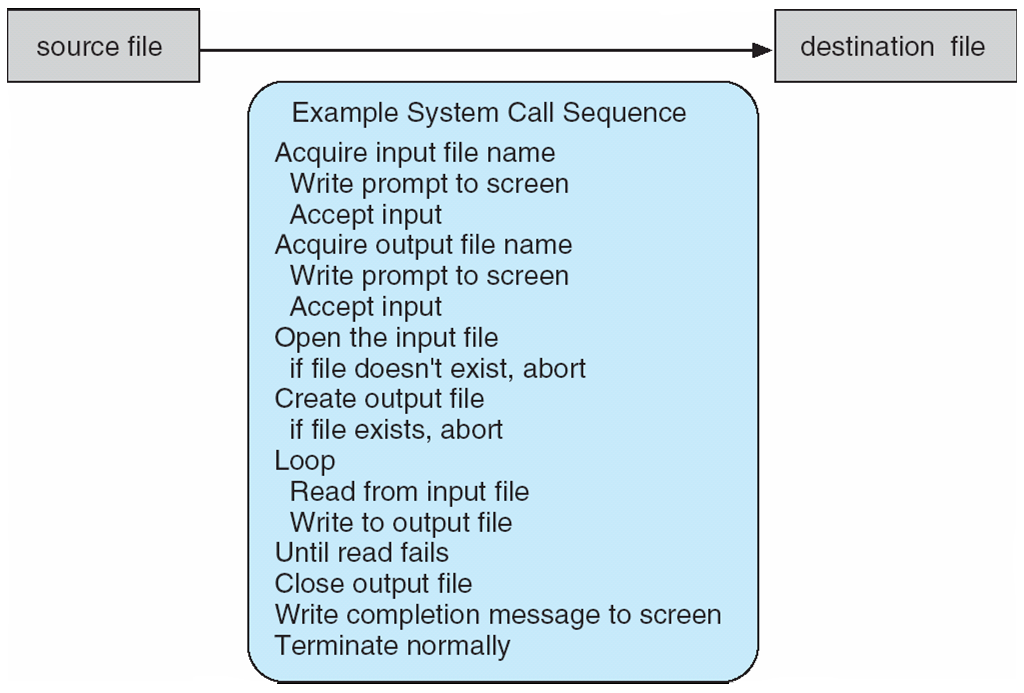
\includegraphics[width=1.0\textwidth]{syscall.png}
%\end{frame}

%\begin{frame}{API -- 系统调用 -- 操作系统之间的关系}
%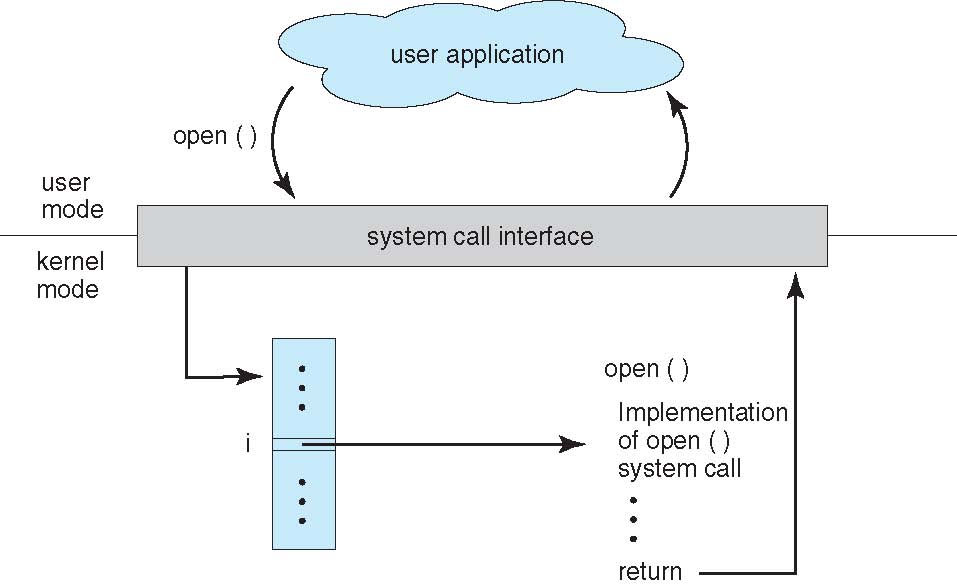
\includegraphics[width=1.0\textwidth]{syscall-os.jpg}
%\end{frame}

%\begin{frame}{API -- 系统调用 -- 操作系统之间的关系: 标准C函数库的例子}
%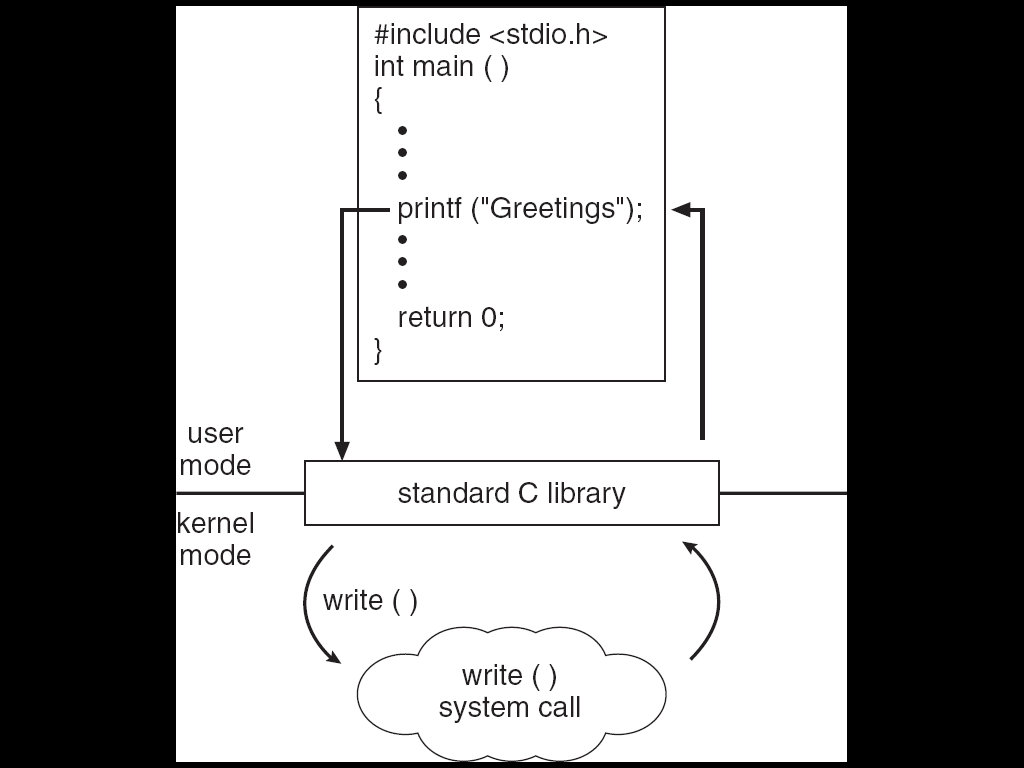
\includegraphics[width=1.0\textwidth]{printf.png}
%\end{frame}

%\begin{frame}{系统调用的例子}
%\end{frame}

\begin{frame}{进程创建, 子进程}
\begin{columns}%[t]
\column{.5\textwidth}
\begin{itemize}
\item 进程可以创建子进程,形成进程树
\item process identifier (pid)
\item 父进程、子进程之间的资源共享
\end{itemize}
\column{.5\textwidth}
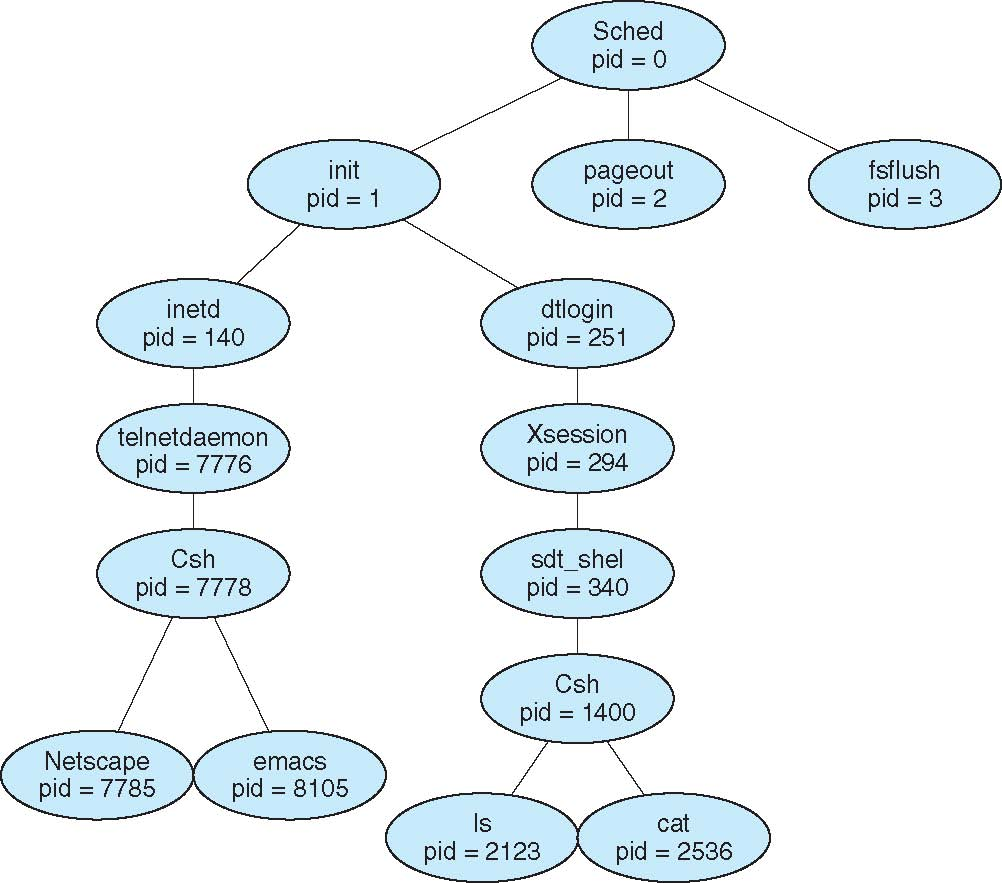
\includegraphics[width=0.9\textwidth]{tree.jpg}
\end{columns}%[t]
\end{frame}

\end{CJK*}
\end{document}
